\begin{center}
	\section{Marco Te\'orico}
\end{center}

\subsection{Extracto}

\noindent
\justify

El extracto es una sustancia procedente de un tejido org\'anico que se compone de \textit{metabolitos} y 
\textit{flavonoides} (ver Figura \ref{flav}). 

\begin{figure}[h!]
\centering
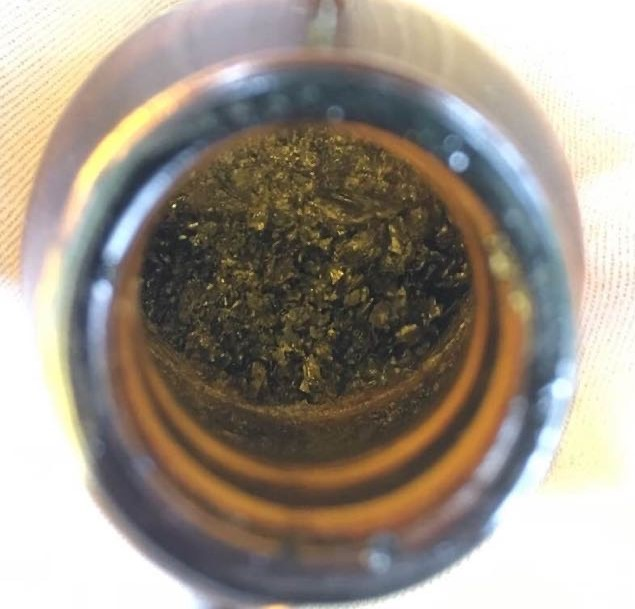
\includegraphics[width=0.4\textwidth]{Images/ext.JPG}
\caption{Extracto de \textit{Lippia alba}.}
\label{extalba}
\end{figure}

\noindent
\justify

Los extractos se utilizan como materias primas para la elaboraci\'on de productos de consumo en diferentes industrias. La actividad biol\'ogica del extracto depende tanto de su procedencia como del tipo de solvente empleado durante el proceso de extracci\'on.

\subsubsection{Flavonoides}

\noindent
\justify

Se trata de sustancias fen\'olicas aisladas de una amplia gama de plantas vasculares, con m\'as de 8000 compuestos conocidos $^{\cite{MartinezFlorez2002}}$.

\begin{figure}[h!]
\centering
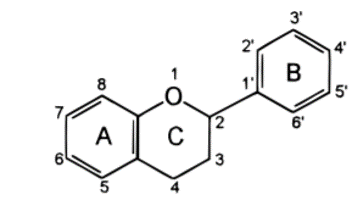
\includegraphics[width=0.5\textwidth]{Images/flavonoide.png}
\caption{Estructura qu\'imica de un flavonoide.}
\label{flav}
\end{figure}

\noindent
\justify

Estos compuestos tienen aplicaciones como: antioxidante, antibacterial, antif\'ungica, insecticida y plagicida$^{\cite{MartinezFlorez2002}}$.

\subsubsection{Plantas end\'emicas}

\noindent
\justify

El tipo de especie define la actividad biol\'ogica del extracto obtenido. Un resumen de las plantas end\'emicas que se procesar\'ian en la biof\'abrica, se puede apreciar en el Cuadro \ref{plantas}.

%\begin{landscape}
\begin{table}[htp!]
\centering
\begin{adjustbox}{max width=0.94\textwidth}
\begin{tabular}{ | l | l | l | l | }
\hline
	\textbf{Especie vegetal} & \textbf{Actividad biol\'ogica} & \textbf{Composici\'on Qu\'imica} & \textbf{Aplicaciones} \\ \hline
	\multirow{2}{*}{\textit{Lippia origanoides}} & \begin{tabular}[c]{@{}l@{}}Actividad \\ antimicrobiana\end{tabular} & \begin{tabular}[c]{@{}l@{}}Carvacrol, \\
$\gamma$-terpineno,\\
timol\end{tabular} & \begin{tabular}[c]{@{}l@{}}Alta actividad \\ antioxidante 
y efectividad \\ contra control de plagas.\end{tabular} \\ \cline{2-4}
	 & Actividad antif\'ungica & \begin{tabular}[c]{@{}l@{}}Timol, O-acetiltimol, \\
O-cimeno\end{tabular} & \begin{tabular}[c]{@{}l@{}}Efectivo contra \\
P. cinnamomi.\end{tabular} \\ \hline
	\textit{Lippia canescens} & \begin{tabular}[c]{@{}l@{}}Baja actividad \\
antiproliferativa \end{tabular}& Flavonoides: Flavonas & N/A \\ \hline
	\multirow{5}{*}{\textit{Turnera diffusa}} & \begin{tabular}[c]{@{}l@{}}Actividad \\antibacteriana\end{tabular} & Extracto de hexano & \begin{tabular}[c]{@{}l@{}}Efectivo contra bacterias \\
grampositivas y \\ gramnegativas\end{tabular} \\ \cline{2-4}
	 & N/A & \begin{tabular}[c]{@{}l@{}}\'oxido de cariofileno,\\
cariofileno,\\
y-cadineno,\\
elemeno,\\
1,8-cineol\end{tabular} & \begin{tabular}[c]{@{}l@{}}Se utiliza como brebaje,\\
ingrediente para licores\end{tabular} \\ \cline{2-4}
	 & N/A & N/A & \begin{tabular}[c]{@{}l@{}}Tratamiento de\\ \'ulceras
g\'astricas. \end{tabular}\\ \hline
	\multirow{3}{*}{\textit{Cordia curassavica}} & \begin{tabular}[c]{@{}l@{}}Actividad \\antibacteriana \\y
antif\'ungica\end{tabular} & \begin{tabular}[c]{@{}l@{}}4-methyl, 4-ethenyl-3-\\
(1-methyl ethenyl)-1-\\
(1-methyl methanol)\\
cyclohexano,\\
$\beta$-Eudesmol,\\
Spathulenol,\\
Cadina\end{tabular} & \begin{tabular}[c]{@{}l@{}}Tratamiento de enferme-\\
dades infecciosas.\end{tabular} \\ \cline{2-4}
	 & Potencial larvicida & \begin{tabular}[c]{@{}l@{}}$\alpha$-pineno,\\
$\beta$-pineno,\\
E-cariofileno,\\
bicyclogermacrene\end{tabular} & \begin{tabular}[c]{@{}l@{}}Efectivo contra larvas del\\
mosquito Ae. Aegypti que\\
transmite el dengue y la \\
fiebre amarilla\end{tabular} \\ \hline
	\multirow{2}{*}{\textit{Psidium sartorianum}} & Actividad antif\'ungica & N/A & N/A \\ \cline{2-4}
	 & \begin{tabular}[c]{@{}l@{}}Actividad \\antiparasitaria\end{tabular} & Pinosotrobin chalcone & N/A \\ \hline
	\textit{Tagetes caracasana} & Actividad antiproliferante & N/A & \begin{tabular}[c]{@{}l@{}}Present\'o efecto nocivo\\ 
contra las c\'elulas \\
cancer\'igenas. \end{tabular} \\ \hline
	\multirow{2}{*}{\textit{Wedelia calycina}} & Actividad antibacteriana & \begin{tabular}[c]{@{}l@{}}Germacren-D,\\
3,3,7,7-tetrametil-5-\\
(2-metil1-propenil)-\\
triciclo [4.1.0.0(2,4)]\\
heptano,\\
$\beta$-sesquifelandreno\end{tabular} & Tratamiento contra la tos. \\ \cline{2-4}
	 & Actividad larvicida & N/A & \begin{tabular}[c]{@{}l@{}}Efectivo contra Aedes \\
aegypti\end{tabular} \\ \hline
	\multirow{3}{*}{\textit{Piper cumanense}} & Actividad antiparasitaria & N/A & \begin{tabular}[c]{@{}l@{}}Tratamiento contra la\\
malaria y la fiebre.\end{tabular} \\ \cline{2-4}
	 & Actividad antif\'ungica & \multirow{2}{*}{\begin{tabular}[c]{@{}l@{}}$\alpha$-pineno,\\
$\beta$-pineno,\\
linanool,\\
germacreno,\\
$\beta$-cariofileno\end{tabular}} & \begin{tabular}[c]{@{}l@{}}Efectivo contra Fusarium \\
oxysporum.\end{tabular} \\ \cline{2-2} \cline{4-4}
	 & Actividad insecticida &  & \begin{tabular}[c]{@{}l@{}}Efectivo contra Sitophilus\\
zeamis y Spodoptera \\
frugiperda. \end{tabular}\\ \hline
\end{tabular}
\end{adjustbox}
\caption{Resumen de algunas plantas end\'emicas de Colombia.}
\label{plantas}
\end{table}
%\end{landscape}

\begin{center}
	\section{M\'etodo MSPD}
\end{center}

\noindent
\justify

El m\'etodo de dispersi\'on de la matriz en fase s\'olida (MSPD, por sus siglas en ingl\'es) ha sido ampliamente utilizado para el estudio de muestras biol\'ogicas. Existen m\'as de 250 publicaciones en las que se emplea este m\'etodo extractivo para el an\'alisis de extractos de distintas naturalezas $^{\cite{barker2007}}$. Esto se debe a la alta eficiencia y bajo costo de este m\'etodo de extracci\'on. 

\noindent
\justify

Consiste, b\'asicamente, de tres etapas (como se puede observar en la Figura \ref{mspd}):

\begin{enumerate}
	\item Maceraci\'on de la muestra con un \textit{agente dispersante} (material particulado, normalmente compuesto de s\'ilice).
	\item Homogenizaci\'on de la muestra macerada en la columna.
	\item Eluci\'on con solvente y filtrado de la mezcla \textit{solvente - extracto}.
\end{enumerate}

\begin{figure}[h!]
\centering
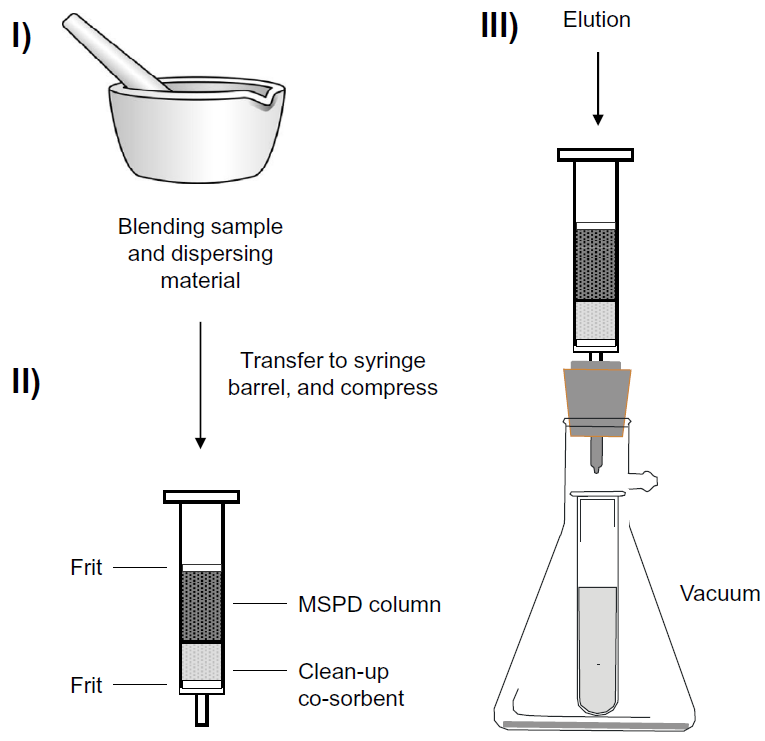
\includegraphics[width=0.8\textwidth]{Images/mspd.PNG}
\caption{M\'etodo MSPD$^{\cite{Capriotti2015}}$.}
\label{mspd}
\end{figure}

\subsection{Factores a considerar en la extracci\'on MSPD}

\noindent
\justify

Hay varios factores a considerar en la extracci\'on MSPD, que incluye:

\begin{enumerate}
	\item \textit{Efecto del tama\~no de part\'icula media:} tama\~nos de part\'icula peque\~nos (entre $3$ - $10 \, \mu m$) requiere de grandes tiempos de eluci\'on y altos gradientes de presi\'on para obtener un flujo adecuado. 
	\item \textit{Agente dispersante:} el uso de silicatos infravalorados, como la arena de r\'io, para la maceraci\'on de muestras presenta resultados diferentes a los reportados con agentes dispersantes como el $C_{18}$ o el $C_8$. A pesar de que el mismo principio de disrupci\'on de la matriz se conserva, debido a la abrasi\'on, es probable que se de una interacci\'on qu\'imica no deseada entre silicatos infravalorados y algunos de los flavonoides del extracto.
	\item \textit{Relaci\'on m\'asica:} la mejor relaci\'on m\'asica reportada en la literatura frecuenta ser una relaci\'on 1 a 4 $^{\cite{barker2007}}$, aunque puede variar de una aplicaci\'on a otra. 
	\item \textit{Solvente:} el vertimiento del solvente en la columna MSPD tiene el fin de aislar analitos espec\'ificos o familias de compuestos. El tipo de solvente, y la polaridad de este, define la composici\'on final del extracto. Existen estudios en donde se ha demostrado un incremento en el rendimiento extractivo al emplear solventes a temperaturas superiores a la temperatura ambiente e inferiores a los $60 \left[ \degree C \right]^{\cite{Vieira2019}}$. 
\end{enumerate}

\subsection{Extracci\'on en fase s\'olida}

\noindent
\justify

El m\'etodo MSPD presenta diferencias claras respecto a la extracci\'on fase s\'olida cl\'asica (SPE, por sus siglas en ingl\'es); entre ellas$^{\cite{barker2007}}$:
\begin{enumerate}
	\item Al emplear el m\'etodo MSPD, se consigue una disrupci\'on completa de la muestra en part\'iculas de reducido tama\~no, incrementando el \'area de extracci\'on. En SPE, la disrupci\'on de la muestra se considera un paso \textit{adicional}, donde muchos de los compuestos se descartan al procesar la muestra para la columna SPE. 
	\item En SPE, la muestra es usualmente absorbida en la parte superior de la columna y no a trav\'es de ella, como en el m\'etodo MSPD.
	\item La interacci\'on f\'isica y qu\'imica de los compuestos del sistema son mayores en el m\'etodo MSPD y diferentes, en diversos sentidos, de aquellos apreciados en el SPE cl\'asico, incluyendo otras formas de cromatograf\'ia l\'iquida.
\end{enumerate}

\newpage

\subsection{Prototipo a escala}

\noindent
\justify

Se han desarrollado estudios experimentales sobre un prototipo a escala de una planta de extracci\'on con capacidad productiva de $1 [kg / bache]$, tres baches al d\'ia. El flujo de trabajo se puede apreciar en la Figura \ref{cadena}.

\begin{figure}[h!]
	\centering
	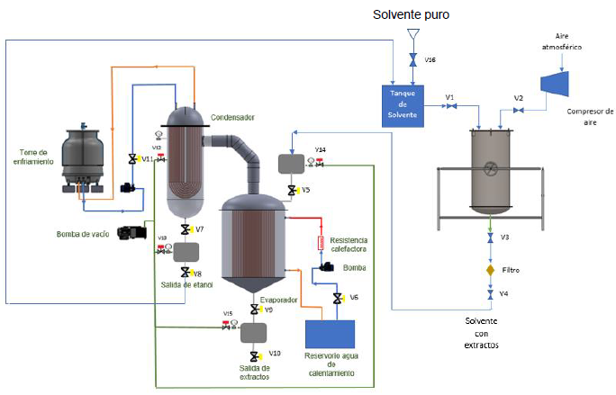
\includegraphics[width=1.1\textwidth]{Images/planta.PNG}
	\caption{Prototipo desarrollado$^{\cite{Proyecto, Patente2018}}$.}
	\label{cadena}
\end{figure}

La invenci\'on desarrollada consiste de:
\begin{itemize}
	\item Molino de bolas dise\~nado como recipiente a presi\'on.
	\item Unidad compresora de aire.
	\item Evaporador.
	\item Condensador.
	\item Sistema de calentamiento de agua por resistencia el\'ectrica.
	\item Torre de enfriamiento.
\end{itemize}




\newpage

\subsection{Sistemas de extracci\'on}

\noindent
\justify

Los m\'etodos industrializados m\'as utilizados en el sector alimenticio emplean extracci\'on \textit{s\'olido - l\'iquido} y con \textit{fluido supercr\'itico (SFE)}$^{\cite{Liadakis2003}}$. 

\subsubsection{Sistemas convencionales $\rightarrow$ \textit{Extracci\'on s\'olido - l\'iquido}}

\noindent
\justify

El dis\~no y selecci\'on del sistema de extracci\'on depende, en gran medida, del compuesto objetivo y de las propiedades f\'isicas tanto del material a extraer como del producto. 

\begin{table}[h!]
\begin{adjustbox}{max width = \textwidth}
\begin{tabular}{|p{2.5cm}|p{2cm}|p{10cm}|}
\hline
\textbf{Modalidad} & \textbf{Tipo} & \textbf{Descripci\'on} \\ \hline
\multirow{3}{*}{\begin{tabular}[c]{@{}l@{}}\textbf{Modo de} \\ \textbf{operaci\'on}\end{tabular}} & Extracci\'on por lotes & La extracci\'on se desarrolla en contenedores llenos con el material s\'olido a extraer. Es ineficiente debido a las paradas de planta por \textit{carga} y \textit{descarga} de material. \\ \cline{2-3}
 & Extracci\'on \textit{semi} continua & Con la idea de incrementar la eficiencia de extracci\'on, se desarrolla una operaci\'on de extracci\'on en serie con m\'ultiples recipientes conectados a la misma l\'inea de solvente, el cual se satura de extracto al pasar por cada uno de ellos. \\ \cline{2-3}
  & Extracci\'on continua & El material a extraer es cargado y descargado de manera continua. Se emplean diferentes sistemas de transporte, tanto para los procesos de filtrado como de inmersi\'on en solvente. No es recomendable para extracciones que requieran presiones distintas a la atmosf\'erica. \\ \hline
\multirow{2}{*}{\begin{tabular}[c]{@{}l@{}}\textbf{Principio de} \\ \textbf{trabajo}\end{tabular}} & Extracci\'on de etapa simple & Emplea un recipiente de una etapa para la extracci\'on por inmersi\'on. La inmersi\'on debe presentar agitaci\'on para tener un m\'argen m\'inimo de eficiencia de extracci\'on. \\ \cline{2-3}
 & Extracci\'on \textit{multi} etapa & Utiliza un sistema de operaci\'on contracorriente (propio de sistemas \textit{semi} continuos). El solvente entra en contacto, primero, con la matriz s\'olida de menor concentraci\'on de extracto hacia el de mayor concentraci\'on.  \\ \hline
\end{tabular}
\end{adjustbox}
\caption{Clasificaci\'on de sistemas de extracci\'on convencionales.}
\label{compara}
\end{table}

\noindent
\justify

Los solventes m\'as empleados consisten en agua, hidrocarburos (como el hexano), alcoholes y las mezclas entre ellos a diferentes proporciones.

\newpage

\noindent
\justify

La tendencia sobre el dise\~no de extractores se enfoca en el mejoramiento de la eficiencia y desempe\~no de extracci\'on. Implica el compromiso entre la \textit{simplicidad} del n\'umero de partes m\'oviles y los sistemas de transporte, bombas y bandas transportadoras, y la \textit{eficiencia} del proceso de eluci\'on del solvente. 

\paragraph{Rotocel}

\noindent
\justify

El extractor \textit{Rotocel} es un sistema de extracci\'on por percolaci\'on desarrollado por Blonox en 1960. Se trata de un tanque giratorio con 18 compartimientos de fondo poroso. El material es rociado en cada celda con diferentes concentraciones de solvente recirculado tipo \textit{contracorriente} (como se obersva en la Figura \ref{rotocel}): el solvente rociado en la primera celda corresponde a solvente con cierto grado de saturaci\'on de extracto (proviene de material procesado de otros compartimientos), mientras que el material de la \'ultima celda se roc\'ia con solvente puro.

\begin{figure}[h!]
	\centering
	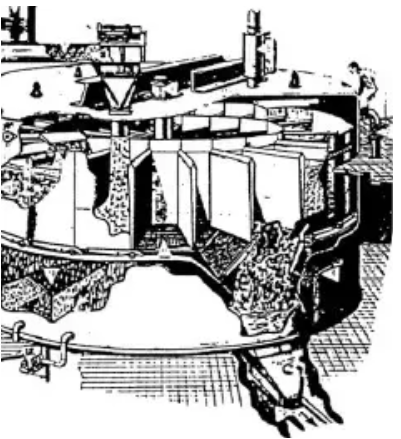
\includegraphics[width=0.5\textwidth]{Images/rotocel.PNG}
	\caption{Extractor Rotocel.}
	\label{rotocel}
\end{figure}

\noindent
\justify

Una rotaci\'on del sistema dura m\'as de una hora, dependiendo de la solubilidad extractiva, y requiere de una energ\'ia rotacional m\'inima debido a que la fuerza de fricci\'on ejercida por el material en cada celda no es de una magnitud considerable. Se conoce como sistema extractor de ``cama profunda", porque cuenta con una profundidad de 1.8 a 3 metros. 

\newpage

\paragraph{Carrousel}

\noindent
\justify

En 1990, el extractor \textit{Carrousel} fue desarrollado mediante la fusi\'on de las licencias Krupp y Extraktionstechnik. Este tipo de extractor puede tener di\'ametros de hasta $15.3 [m]$.

\begin{figure}[h!]
	\centering
	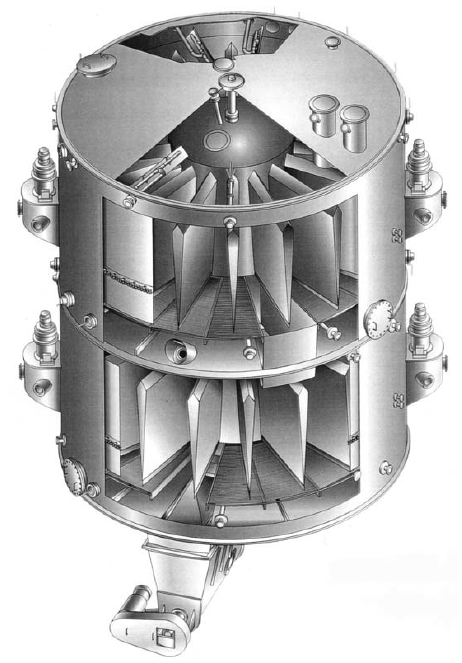
\includegraphics[width=0.4\textwidth]{Images/carrousel.PNG}
	\caption{Interior de un extractor tipo carrousel de doble piso$^{\cite{Liadakis2003}}$.}
	\label{carrousel}
\end{figure}

\noindent
\justify

Presenta el mismo principio de funcionamiento que el sistema de extracci\'on tipo Rotocel, con la diferencia de que el marco de los compartimientos de extracci\'on gira sobre una bandeja de tamiz est\'atica; estructura apreciada en la Figura \ref{tamiz}. 

\begin{figure}[h!]
	\centering
	\begin{subfigure}[b]{0.48\textwidth}
		\centering
		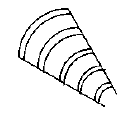
\includegraphics[width=0.5\textwidth]{Images/Original.PNG}
	\caption{Segmento original conc\'entrico.}
	\end{subfigure}
	\hfill
	\begin{subfigure}[b]{0.5\textwidth}
		\centering
		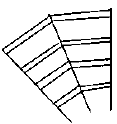
\includegraphics[width=0.48\textwidth]{Images/Actual.PNG}
	\caption{Segmento actual.}
	\end{subfigure}
	\caption{Segmento del fondo de la bandeja de tamiz de un extractor Carrousel$^{\cite{Liadakis2003}}$.}
	\label{tamiz}
\end{figure}

\noindent
\justify

De esta manera, se mejora la transferencia de masa debido a que las part\'iculas se mantinen en constante movimiento.

\paragraph{Pretratamiento}

\noindent
\justify

La eficiencia de extracci\'on est\'a directamente relacionada con la preparaci\'on del material s\'olido a extraer. Peque\~nos tama\~nos de part\'icula son ventajosos debido a la baja resistencia a la difusi\'on entre part\'iculas. Sin embargo, conseguir tama\~nos de part\'icula cercanos al polvo $\left( < 200 \left[ \mu m \right] \right)$ involucra grandes esfuerzos en procesos de trituraci\'on y molienda. Es com\'un emplear como \textbf{pretratamiento mec\'anico} sistemas de molienda de operaci\'on continua; entre ellos: \textit{molinos de rodillos} y \textit{molinos de martillos}, como se aprecia en la Figura \ref{pret}.

\begin{figure}[h!]
	\centering
	\begin{subfigure}[b]{0.5\textwidth}
		\centering
		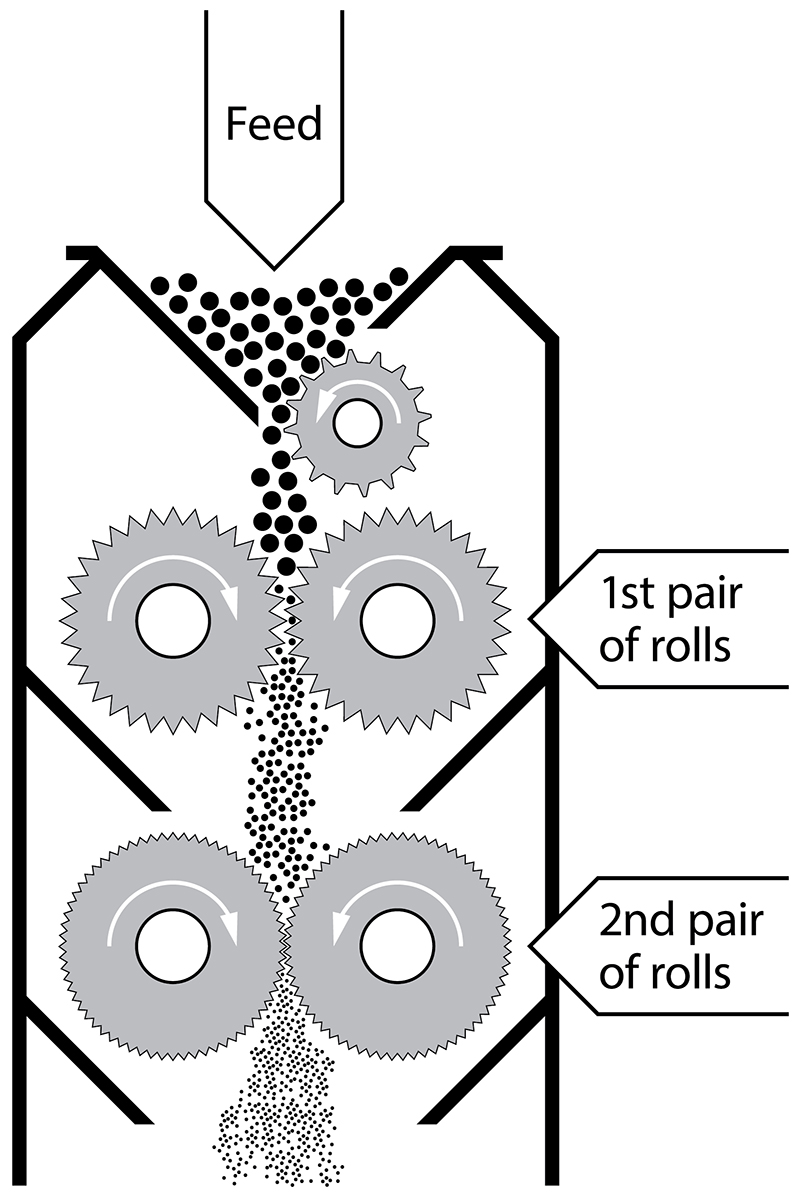
\includegraphics[width=0.7\textwidth]{Images/Rodilloss.png}
	\caption{Molino de rodillos.}
	\end{subfigure}
	\hfill
	\begin{subfigure}[b]{0.5\textwidth}
		\centering
		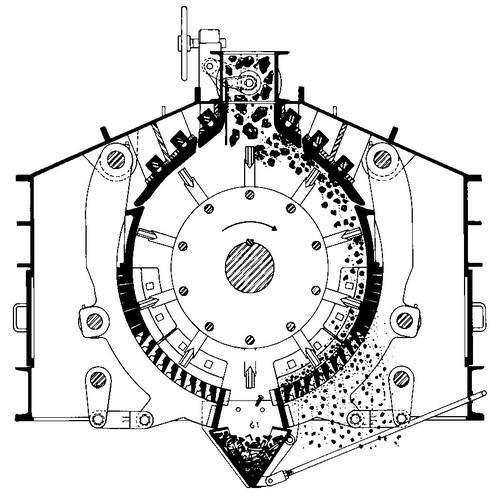
\includegraphics[width=0.9\textwidth]{Images/Martillos.jpg}
	\caption{Molino de martillos.}
	\end{subfigure}
	\caption{Sistemas de pretratamiento mec\'anico.}
	\label{pret}
\end{figure}

\noindent
\justify

En la industria alimenticia es com\'un realizar un \textbf{pretratmiento t\'ermico} para incrementar la eficiencia extractiva durante la producci\'on de aceites con altos valores proteicos, entre ellos: semillas de algod\'on, soja, semillas de s\'esamo y man\'i. Este tratamiento consiste mantener el material solido cerca del $10 \%$ de humedad a temperaturas de $90 - 95 \degree C$.

\paragraph{Recuperaci\'on del solvente}

\noindent
\justify

Una vez obtenida la mezcla solvente - extracto es necesario separarlos a trav\'es de procesos de destilaci\'on. Una vez obtenido el extracto, se pueden realizar procesos de extracci\'on posteriores para limpiarlo de compuestos indeseados, enriquecerlo de otros compuestos o para desarrollar una modificaci\'on qu\'imica.

\subsubsection{Extracci\'on con Fluido Supercr\'itico (SFE)}

\noindent
\justify

La extracci\'on mediante fluido supercr\'itico, especialmente la extracci\'on con dioxido de carbono $\left(CO_2 \right)$, est\'a establecida a una escala industrial y presenta una amplia gama de aplicaciones, entre ellas: producci\'on de caf\'e descafeinado; extracto de l\'upulo; y producci\'on de ingredientes naturales provenientes de hierbas, ra\'ices y aceites esenciales.

\noindent
\justify

El sistema de extracci\'on con fluido supercr\'itico se puede apreciar en la Figura \ref{co2} y consiste de un sistema de presurizaci\'on, un recipente a presi\'on donde ocurre la extracci\'on, otro donde se realiza la separaci\'on y recuperaci\'on del solvente y un par de intercambiadores de calor.

\begin{figure}[h!]
	\centering
	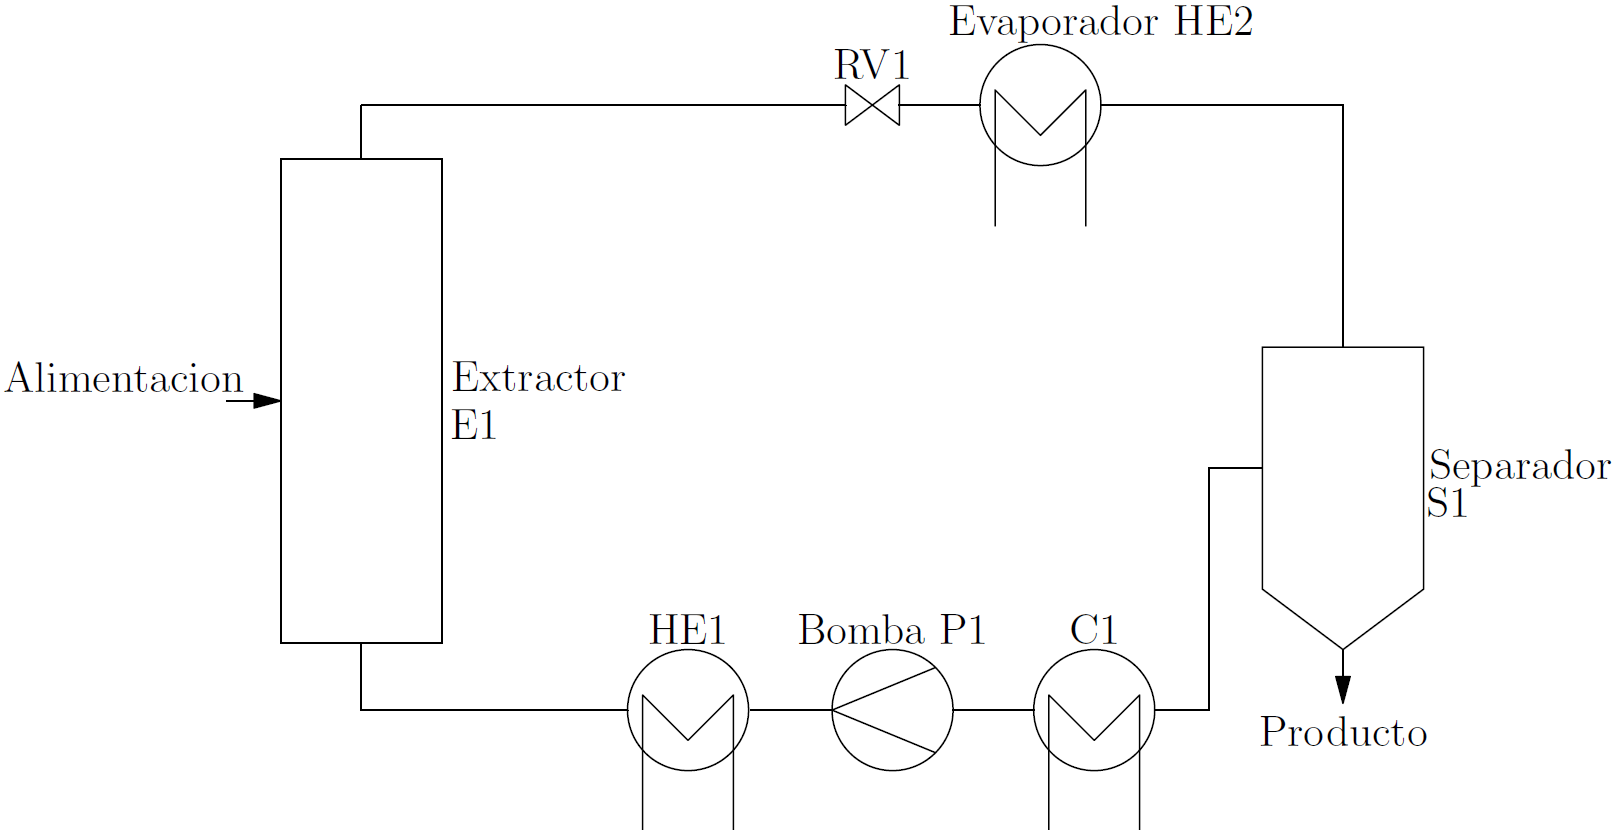
\includegraphics[width=\textwidth]{Images/SFE-CO2/Equipos.PNG}
	\caption{Flujo de trabajo de la extracci\'on con $CO_2$ supercr\'itico.}
	\label{co2}
\end{figure}

\noindent
\justify

El diagrama termodin\'amico del proceso se puede apreciar en la Figura \ref{termo}, del cual se pueden desarrollar balances energ\'eticos.

\begin{figure}[h!]
	\centering
	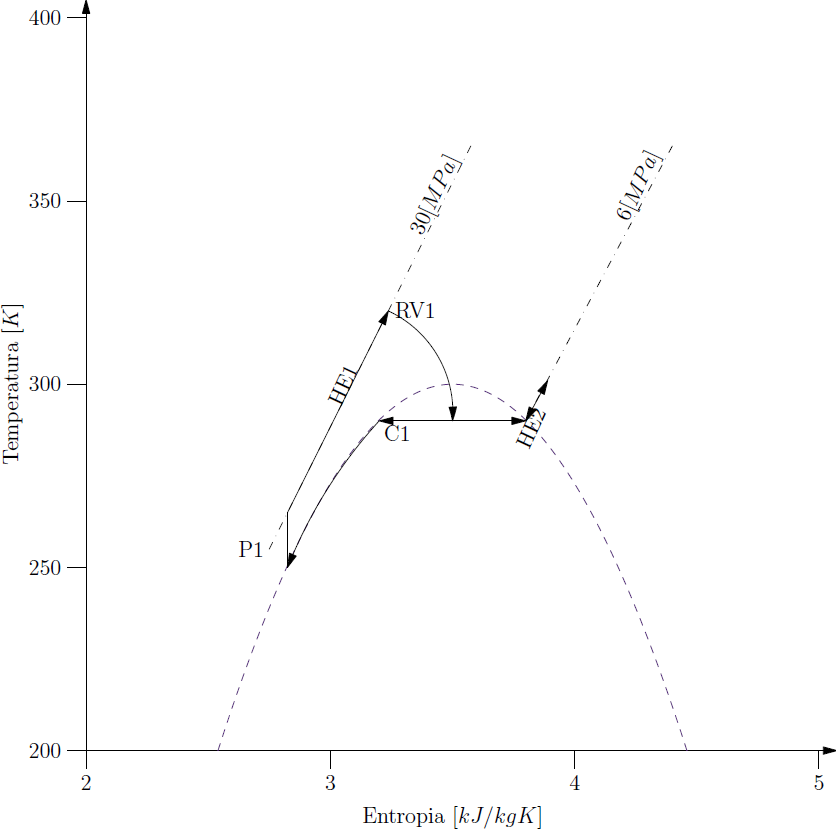
\includegraphics[width=\textwidth]{Images/SFE-CO2/TermoCO2.PNG}
	\caption{Diagrama termodin\'amico T-S.}
	\label{termo}
\end{figure}

\noindent
\justify

Despu\'es de entrar a la zona de l\'iquido saturado en el chiller \textit{C1}, el fluido es lugo comprimido por la bomba \textit{P1}. El incremento de presi\'on se produce de manera casi reversible (isentr\'opicamente). El calentador \textit{HE1} incrementa la temperatura del fluido hasta la temperatura de extracci\'on. Debido a la expansi\'on adiab\'atica que ocurre en la v\'alvula \textit{RV1}, por el efecto Joule-Thompson, el di\'oxido de carbono se enfr\'ia hasta llegar a las condiciones de saturaci\'on. Para facilitar la separaci\'on entre el extracto y el solvente $\left(CO_2 \right)$, el fluido se evapora completamente justo antes de entrar al separador \textit{S1} al pasar por el evaporador \textit{HE2}.



\input{DEMFVM}



